%追加すべき事項
% - ? lossの図と説明
% - ? 追加実験
% - 考察の増強
% - 方法とモデルの増強
\chapter{提案手法}

本章では、提案手法の説明を行う。

\section{提案手法の目標}

提案手法の目標は、提案モデルとなるニューラルネットワークを用い、音の高さと大きさを維持したままでギターの単音からハープの単音への音色の変換を行うことである。また、単音とはある楽器を用いてある高さの一音を鳴らした時に出力される音として定義する。ここで、ほとんどの単音は複数の周波数成分の合成波であり、音の高さは最も低い周波数成分の音~(基音)~の高さである。また、音色の違いは基音より高い音~(上音)~の音波の組み合わせの違いに起因する。

\section{音の表現}

44100~Hzのサンプリング周波数でサンプリングを行った1秒の音響信号を音の表現として使用した。また、量子化ビット数は16ビット、チャンネル数は1である。したがって、本研究で用いる音は44100の長さを持つ16ビット整数の一次元配列として表現される。

\section{提案モデル}
\label{sec:proposed}

本研究では、Pix2pix~\cite{pix2pix}を元に生成モデルと識別のいずれにも条件として変換元の音を入力することで音色の変換を行うGANを提案モデルとして作成した~(\prettyref{fig:pr_model})~。

\begin{figure}[b]
\centering
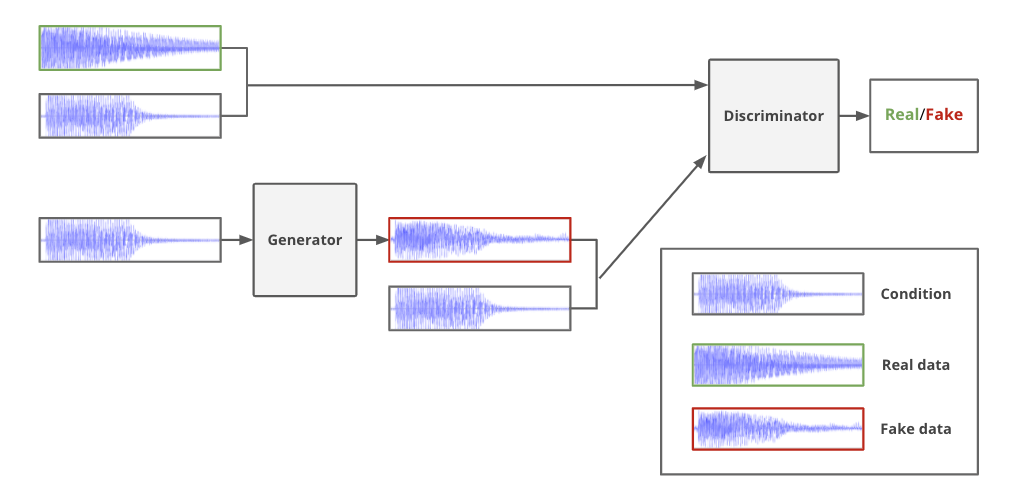
\includegraphics[width=0.75\columnwidth]{figure/pr_model.png}
\caption[本研究の提案モデル]{提案モデル}
\label{fig:pr_model}
\end{figure}

%ここで改ページ
\clearpage

\subsection{生成モデル}

生成モデルには1つのスキップコネクションを持つEncoder-Decoder型のネットワークを用いた。また、入力は条件となる変換元の音波である~(\prettyref{fig:pr_gen})~。また、このモデルでは決定論的に音を生成するために生成モデルの入力にノイズを使用していない。

\subsection{識別モデル}

識別モデルには一般的なCNNを用いた。また、出力は最終層の特徴量マップの平均値である~(\prettyref{fig:pr_dis})~。

\begin{figure}[b]
\centering
\begin{minipage}[b]{0.48\columnwidth}
\centering
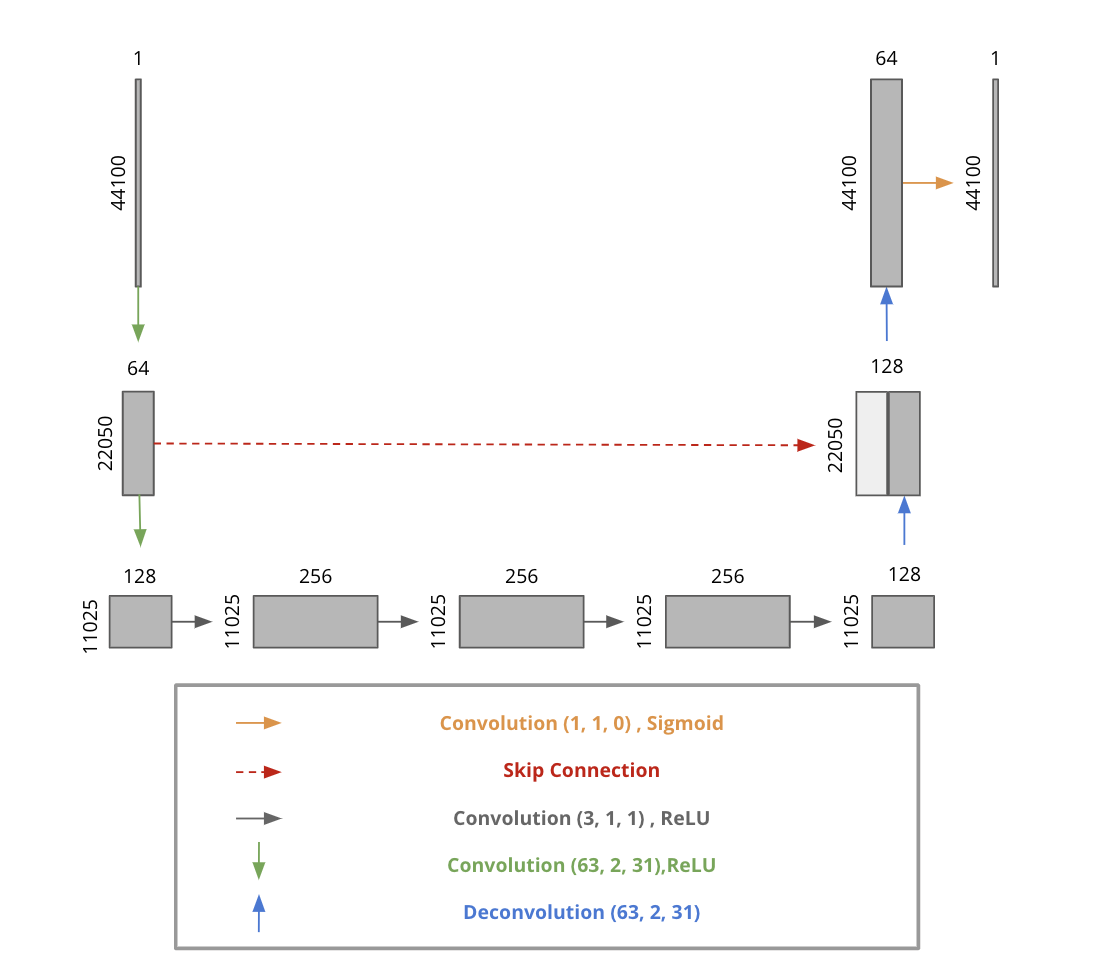
\includegraphics[width=\columnwidth]{figure/pr_generator.png}
\subcaption[本研究の生成モデル]{生成モデルのネットワーク}
\label{fig:pr_gen}
\end{minipage}
\begin{minipage}[b]{0.48\columnwidth}
\centering
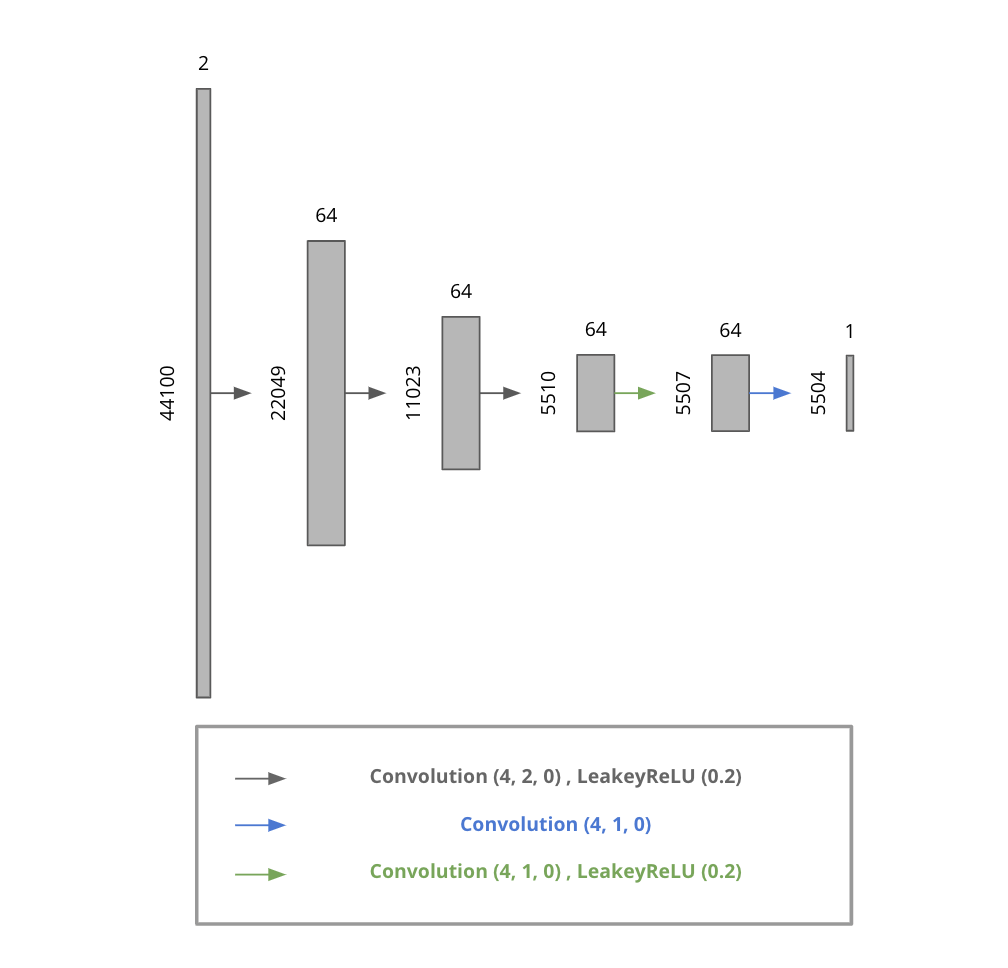
\includegraphics[width=\columnwidth]{figure/pr_discriminator.png}
\subcaption[本研究の識別モデル]{識別モデルのネットワーク}
\label{fig:pr_dis}
\end{minipage}
\caption[本研究の生成モデルと識別モデル]{~\cite{u-net}のFigure~1を参考に作成した。灰色の箱は特徴量マップであり、箱の上側にチャンネル数を示し、箱の左側に特徴量マップとなる一次元配列の長さを示す。また、ネットワーク構造の下の囲みの中にそれぞれの矢印の操作を示す。ConvolutionとDeconvolutionについては~(カーネルサイズ、パディング数、ストライド)~としてそれぞれの値を示し、LeakeyReLUについては負の実数の定義域での一次関数の傾きの値を示す。}
\label{fig:pr}
\end{figure}

\chapter{実験}

本章では、データセットと実験方法の説明を行った後、実験結果の考察を行う。

\section{データセット}

データセットとして1秒のギターとハープの音を88組用いた。また、この88音は音の大きさが等しいものと仮定した。そして、音の高さとしてはA0$\sim$C8の88音の半音を選んだ。これらは一般的な88鍵のピアノのそれぞれの鍵盤の音に対応する~(\prettyref{fig:piano})~。

\subsection{音階表記}

本実験では西洋音楽の12音階表記を音階表記に用いる。この表記では、$C,C^{\sharp},D,D^{\sharp},E,F,F^{\sharp},G,$\\
$G^{\sharp},A,A^{\sharp},B$の12段階の音の高さの集合をオクターブとして定める。そして、それぞれのオクターブに番号を振り、440~Hzの音をA4と定めることで音の高さの絶対的な表記を可能にしている。

\section{実験方法}

本節では実験方法の説明を行う。

\subsection{提案モデルの表現力の評価実験}

提案モデルの表現力を評価する実験を行った。具体的には、用意した88音を学習データと評価データのいずれでも使用し、同じ高さの音の間での変換の実験を行った。

\subsection{提案モデルの汎化能力の評価実験}

任意の高さと大きさの音を学習データとして用意するのは不可能であるため、提案モデルの汎化能力を評価する必要がある。ここでは、88音のうち3/4を学習データ、1/4を評価データとする4分割交差検定により実験を行った。また、データセットの分割方法は\prettyref{app:split}に示す。

\begin{figure}[b]
\centering
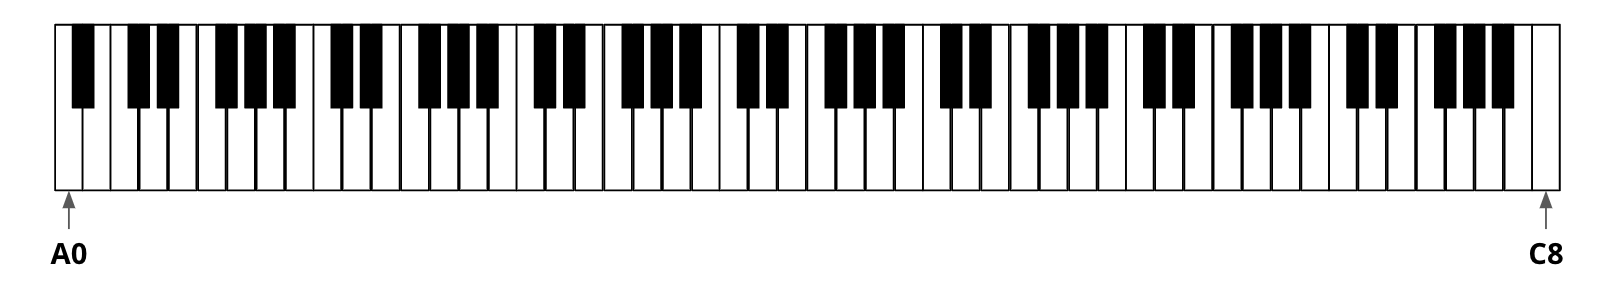
\includegraphics[width=0.7\columnwidth]{figure/piano.png}
\caption{88鍵のピアノの鍵盤}
\label{fig:piano}
\end{figure}

%ここで改ページ
\clearpage

\subsection{データ拡張}

各エポックの任意の学習データの振幅を無作為化することでデータ拡張を行った。具体的には、学習前に乱数のシードを固定した後に一様乱数により$0.3\sim1.0$の乱数を生成した。また、これにより88音と小さいサイズのデータセットへの過学習を防ぐことを期待した。

\subsection{提案モデルの学習}

モデルの学習時のパラメータの更新は\prettyref{sec:grad}にある勾配降下法を利用して行う。また、勾配降下法としてはAdam~\cite{Adam}を用い、ハイパーパラメータは\prettyref{app:params}に示す。

\subsection{評価方法}

生成モデルの出力が音の高さ及び音の大きさを保持したまま変換先のハープの音の音色に変換できているかという観点から音波の観察と音の聴き取りにより評価を行った。また、音色の変換対象としてギターとハープを選んだ理由は、弦楽器という共通点を持ちながらも音波の観察と音の聴き取りの評価により十分に異なると判定できると考えたからである。

\section{実験結果}

実験結果の考察を本節では行う。また、実験結果に記載する波形の図は三つの波形を上から並べている。これらは上から順に、変換元のギターの波形、生成モデルの出力波形、変換先のハープの波形、である。そして、本節には一部の音波のみを記載し、\prettyref{app:result}に他の音波の波形を記載する。

\subsection{概要:提案モデルの表現力の評価実験}

提案モデルの表現力の評価実験を行ったところ、実験結果は二つに大別された。

\subsubsection{ハープの音を表現できた場合}

88音のうち86音はハープの音を表現することができた。~(\prettyref{fig:88_88_good1})~。また、特にC4からD5$\sharp$は目標のハープの音に極めて近い音を生成することができた~(\prettyref{fig:88_88_good2})~。これらの音は上音が少ないため、他の音と比べて表現が容易であったと推察される。

\begin{figure}[b]
\centering
\begin{minipage}{0.48\columnwidth}
\centering
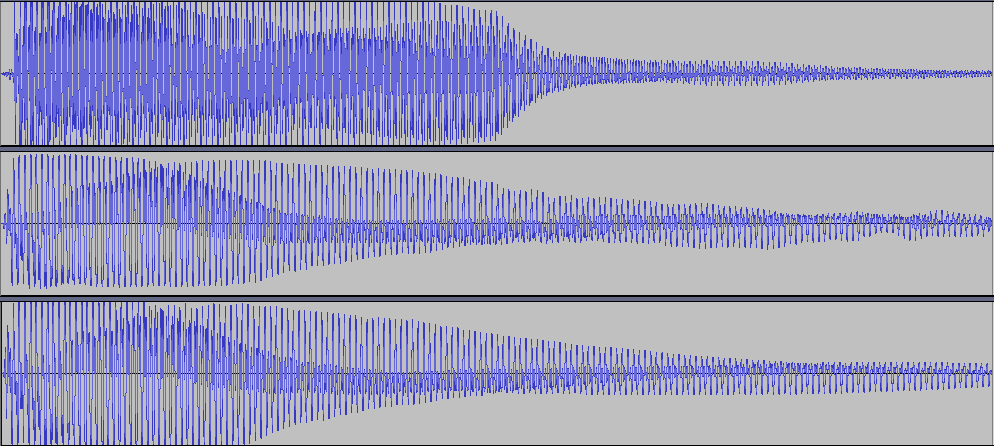
\includegraphics[width=0.9\columnwidth]{figure/88_88/f3.png}
\caption[F3の音波]{F3の0.800秒から1.000秒までの音波}
\label{fig:88_88_good1}
\end{minipage}
\begin{minipage}{0.48\columnwidth}
\centering
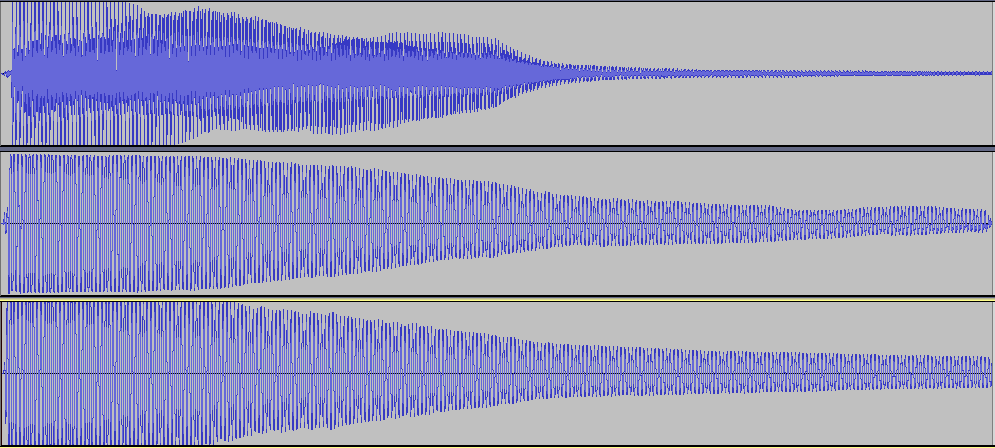
\includegraphics[width=0.9\columnwidth]{figure/88_88/c4.png}
\caption[C4の音波]{C4の0.200秒から0.300秒までの音波}
\label{fig:88_88_good2}
\end{minipage}
\end{figure}

%ここで改ページ
\clearpage

\subsubsection{ハープの音を表現できなかった場合}

D7$\sharp$とE7の2音は音の高さは維持できたものの、ハープの音を十分に表現できなかった~(\prettyref{fig:88_88_bad1}と\prettyref{fig:88_88_bad2})~。いずれの音についてもハープの音波の振動が安定しておらず、この不安定さを表現することはできなかった。また、他の高音においても振動が不安定なものが見られたため、高音において安定したデータセットをハープで生成するのが難しいと推察される。

\begin{figure}[b]
\centering
\begin{minipage}{0.48\columnwidth}
\centering
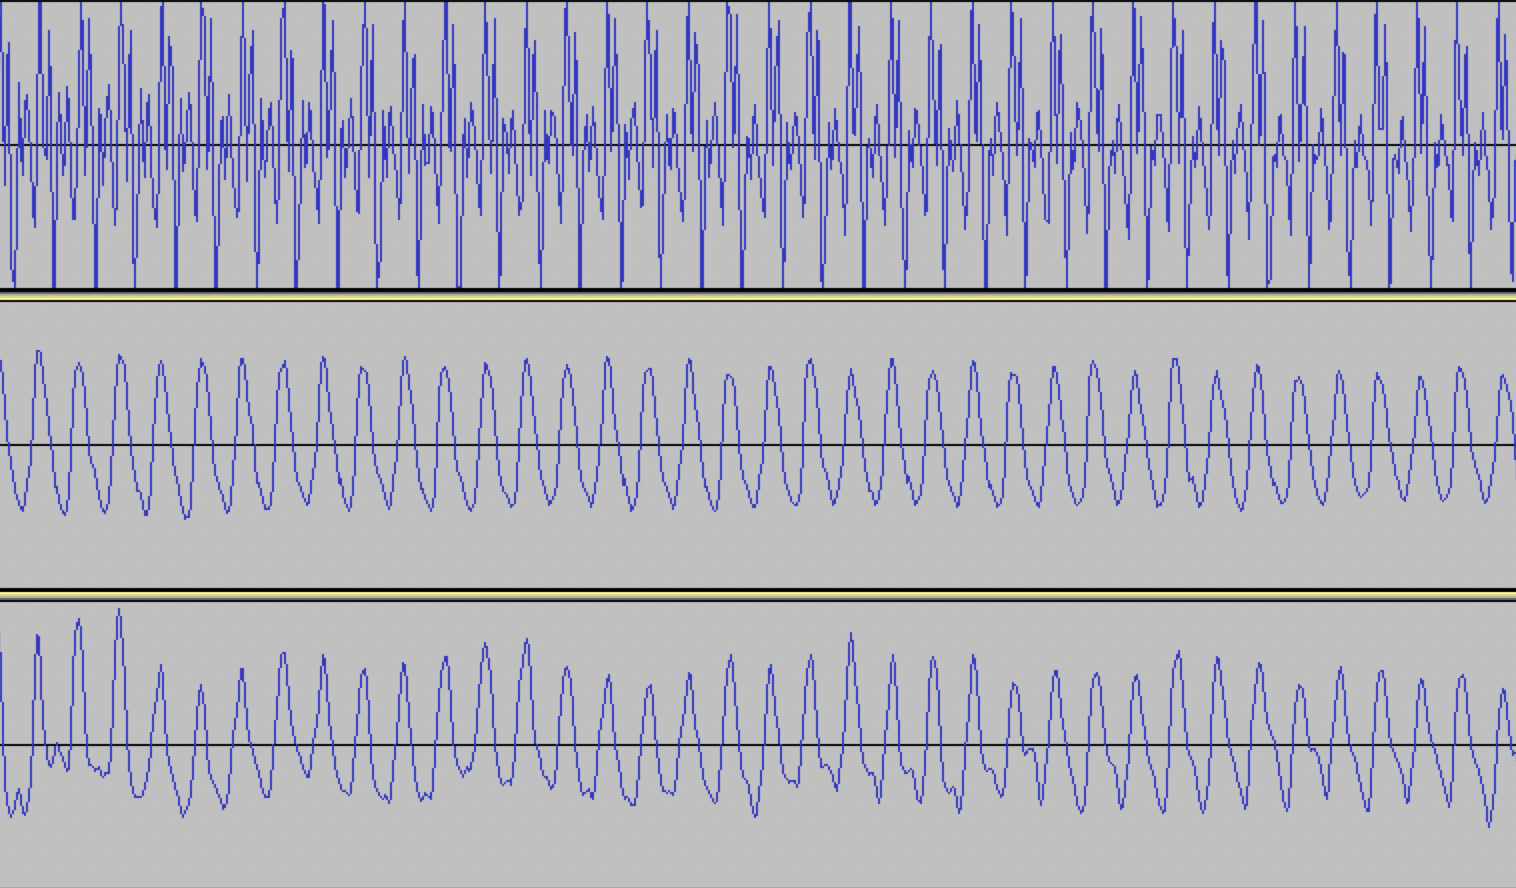
\includegraphics[width=0.9\columnwidth]{figure/88_88_det/d7s_0550_0700.png}
\caption[D7$\sharp$の音波]{D7$\sharp$の0.055秒から0.070秒までの音波}
\label{fig:88_88_bad1}
\end{minipage}
\begin{minipage}{0.48\columnwidth}
\centering
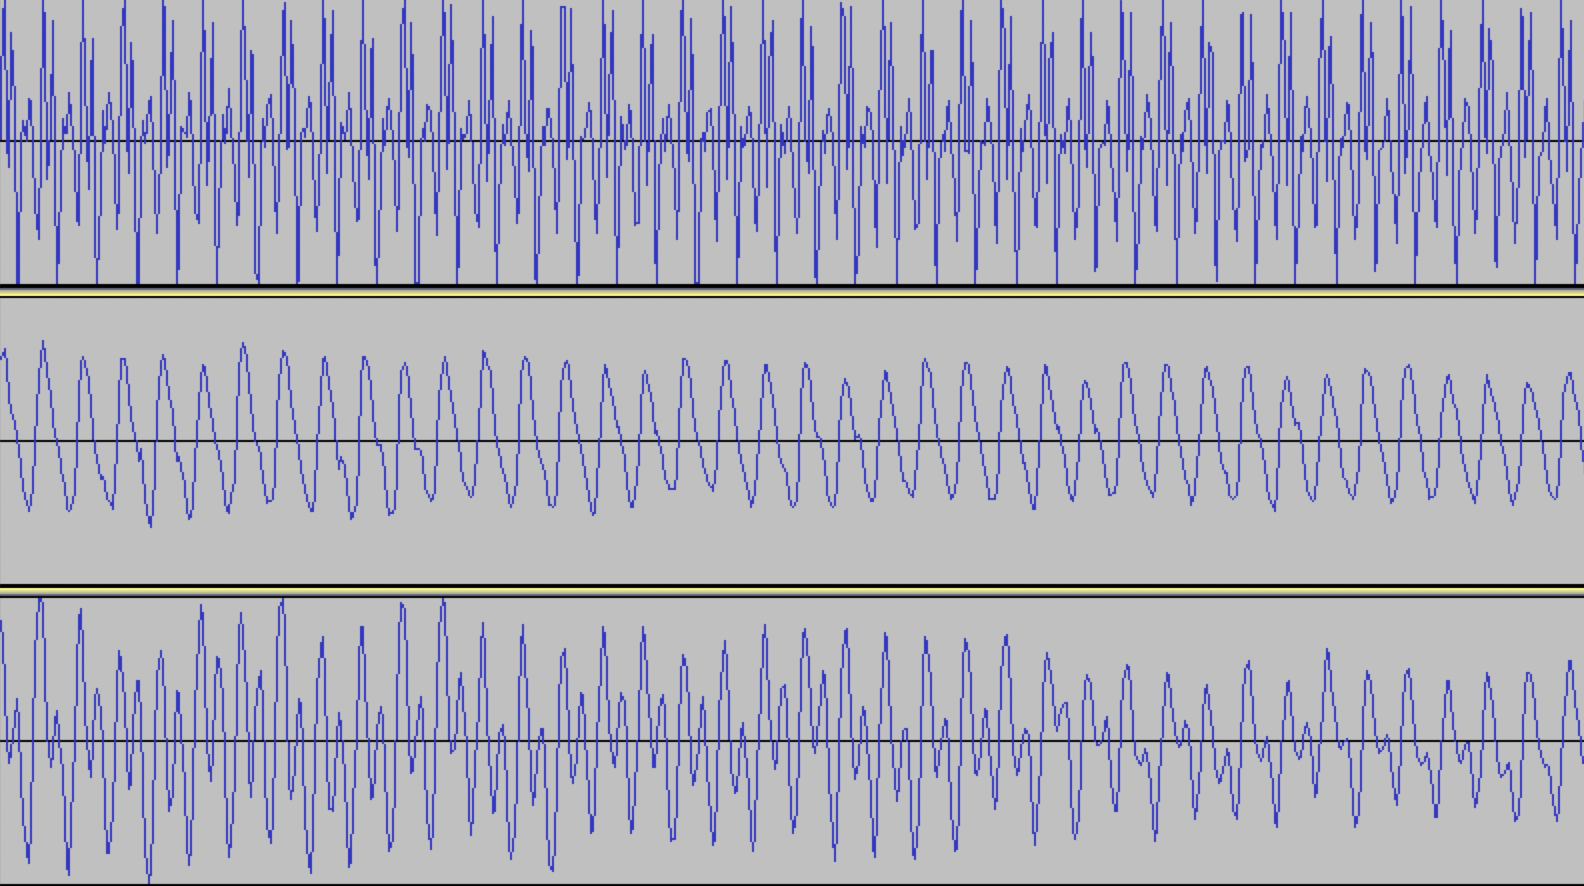
\includegraphics[width=0.9\columnwidth]{figure/88_88_det/e7_0550_0700.png}
\caption[E7の音波]{E7の0.055秒から0.070秒までの音波}
\label{fig:88_88_bad2}
\end{minipage}
\end{figure}

\subsection{概要:提案モデルの汎化能力の評価実験}

提案モデルの汎化能力の評価実験を行ったところ、実験結果は三つに大別された。

\subsubsection{ハープの音を表現できた場合}

D4,D4$\sharp$,G4,F5,F5$\sharp$の5音はハープの音を表現することができた~(\prettyref{fig:66_22_near})~。これらの高さの音では、提案モデルの表現力の評価実験の際にも特に綺麗なハープの音を表現できており、上音が少ないほど表現が容易であるという推察を示していると思われる。

\subsubsection{ハープの音を表現できず音の高さも維持できなかった場合}

C7,D7$\sharp$,E7,F7$\sharp$,G7,G7$\sharp$,A7,B7,C8の9音は音の高さも維持することができず、騒音が生成された~(\prettyref{fig:66_22_bad4})~。これらの高さの音では提案モデルの表現力の評価実験の際にもハープの音を表現できておらず、やはり高音域における安定したデータセットの作成は難しいと考えられる。また、高音域では周波数が高くノイズの影響が大きく出たとも考えられる。

\begin{figure}[b]
\centering
\begin{minipage}{0.48\columnwidth}
\centering
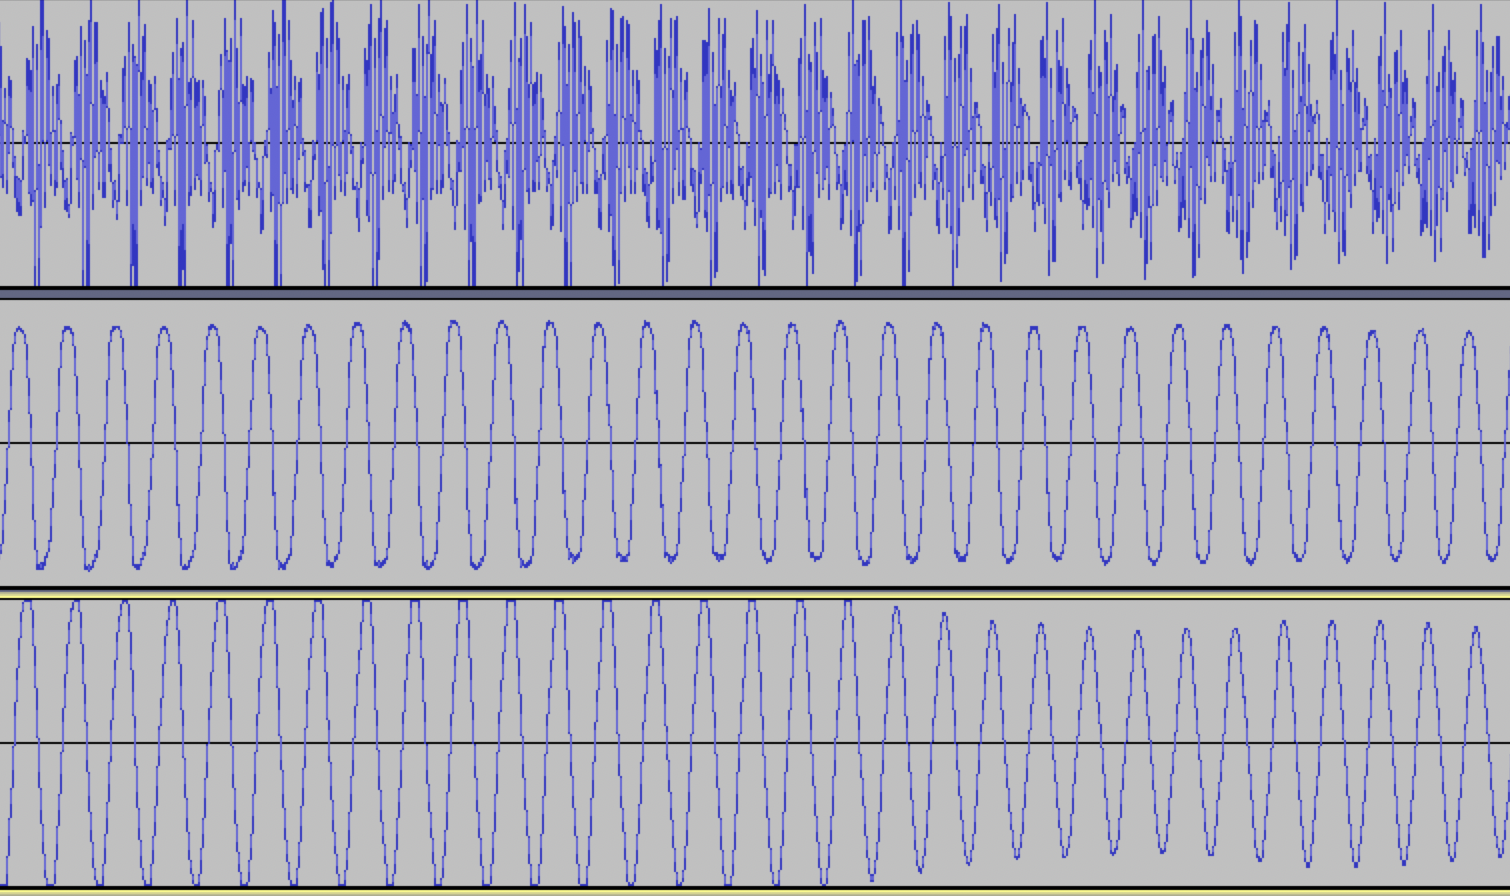
\includegraphics[width=0.85\columnwidth]{figure/66_22_det/d4s_0100_0200.png}
\caption[D4$\sharp$の音波]{D4$\sharp$の0.100秒から0.200秒までの音波}
\label{fig:66_22_near}
\end{minipage}
\begin{minipage}{0.48\columnwidth}
\centering
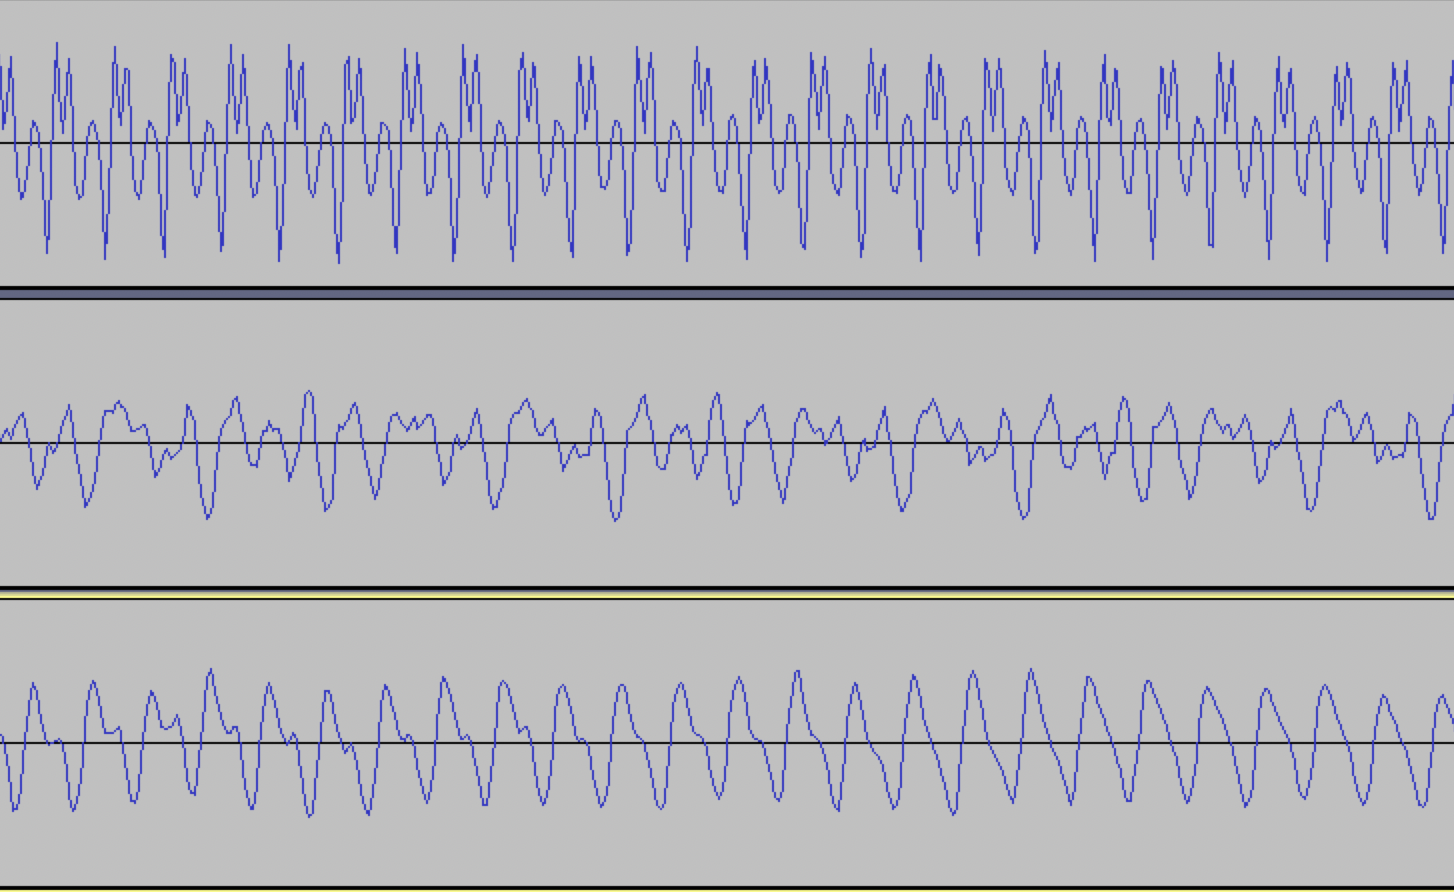
\includegraphics[width=0.85\columnwidth]{figure/66_22_det/d7s_0100_0110.png}
\caption[D7$\sharp$の音波]{D7$\sharp$の0.1700秒から0.110秒までの音波}
\label{fig:66_22_bad4}
\end{minipage}
\end{figure}

%ここで改ページ
\clearpage

\subsubsection{ハープの音を表現できず音の高さを維持できた場合}

14音を除く74音については音の高さは維持できているもののハープの音を表現することができなかった~(\prettyref{fig:66_22_bad1}、\prettyref{fig:66_22_bad2})~。これらの音では、音波が安定した振動をせず上音の成分がハープよりも多い音波が多く観測された。また、これらの高さの音は提案モデルの表現力の評価実験の際には表現することができていたため、提案モデルの汎化能力の低さが明らかになった。

\begin{figure}[b]
\centering
\begin{minipage}{0.48\columnwidth}
\centering
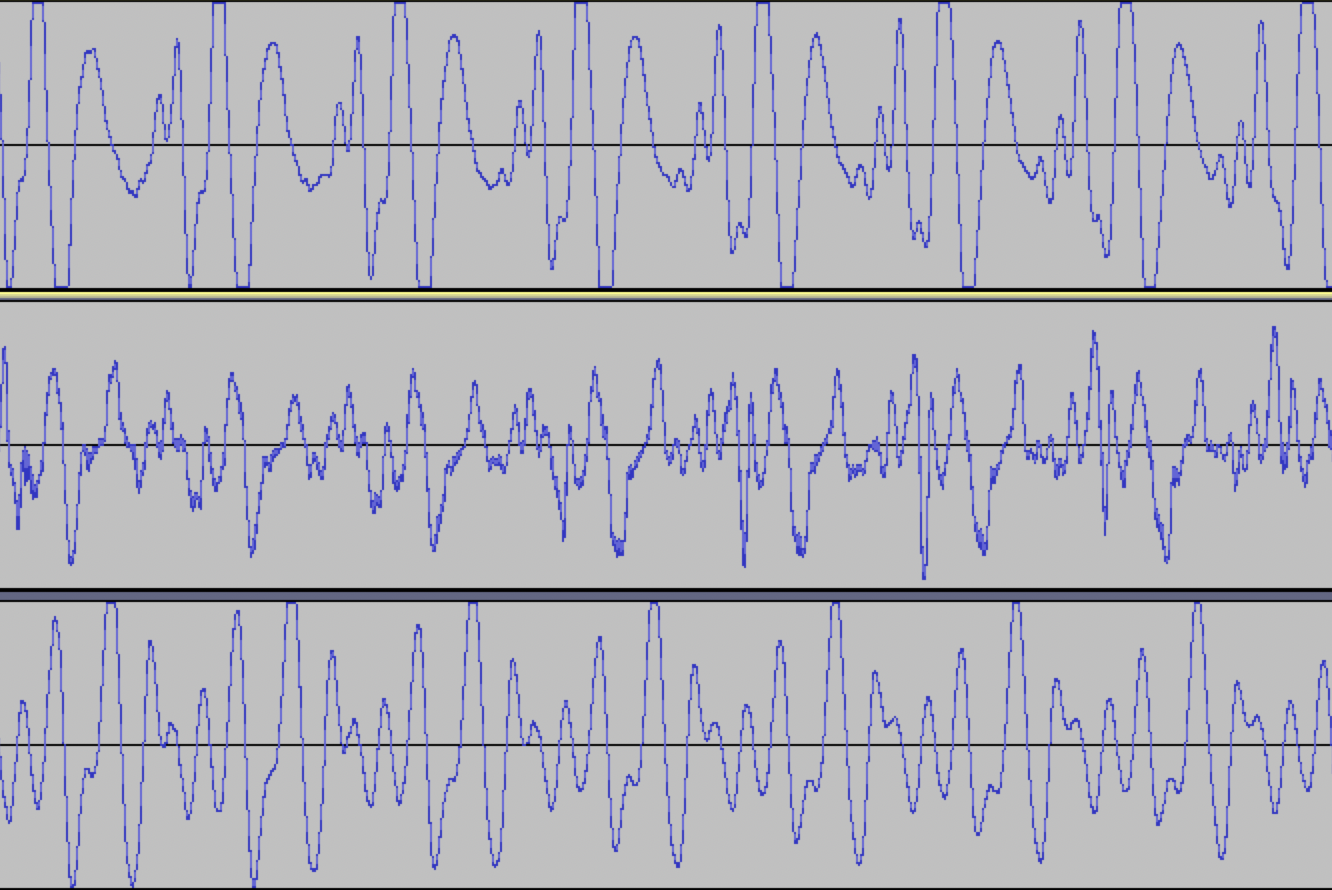
\includegraphics[width=0.75\columnwidth]{figure/66_22_det/d1_0300_0500.png}
\caption[D1の音波]{D1の0.300秒から0.500秒までの音波}
\label{fig:66_22_bad1}
\end{minipage}
\begin{minipage}{0.48\columnwidth}
\centering
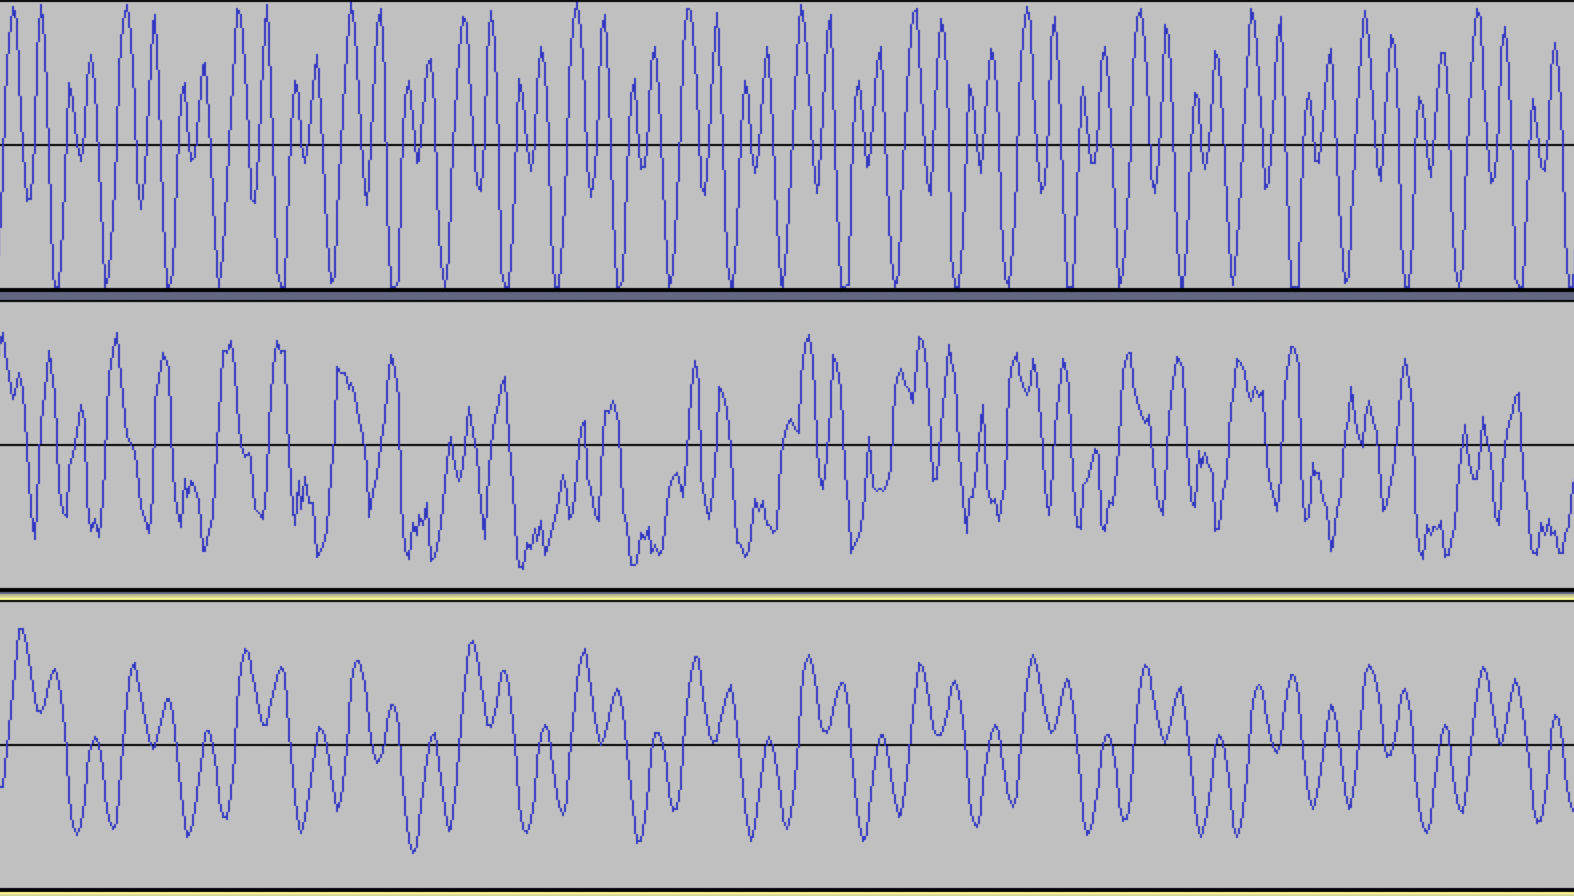
\includegraphics[width=0.85\columnwidth]{figure/66_22_det/f6_0070_0080.png}
\caption[F6の音波]{F6の0.070秒から0.080秒までの音波}
\label{fig:66_22_bad2}
\end{minipage}
\end{figure}

\subsection{課題}
\label{sec:result}

提案モデルの表現力の評価実験の実験結果から四つの課題が明らかになった。

\subsubsection{音の減衰の表現}

振動の減衰を表現できていない音がいくつかあった。これらの音のうち、E2以下の低音域ではハープとは全く異なる波形で減衰し~(\prettyref{fig:88_88_reduce1})~、A6以上の高音域ではほとんど振動が見られなかった~(\prettyref{fig:88_88_reduce2})~。また、提案モデルでは表現力が足りず微小な振動の学習が難しいためであると考えられる。

\begin{figure}[b]
\centering
\begin{minipage}{0.48\columnwidth}
\centering
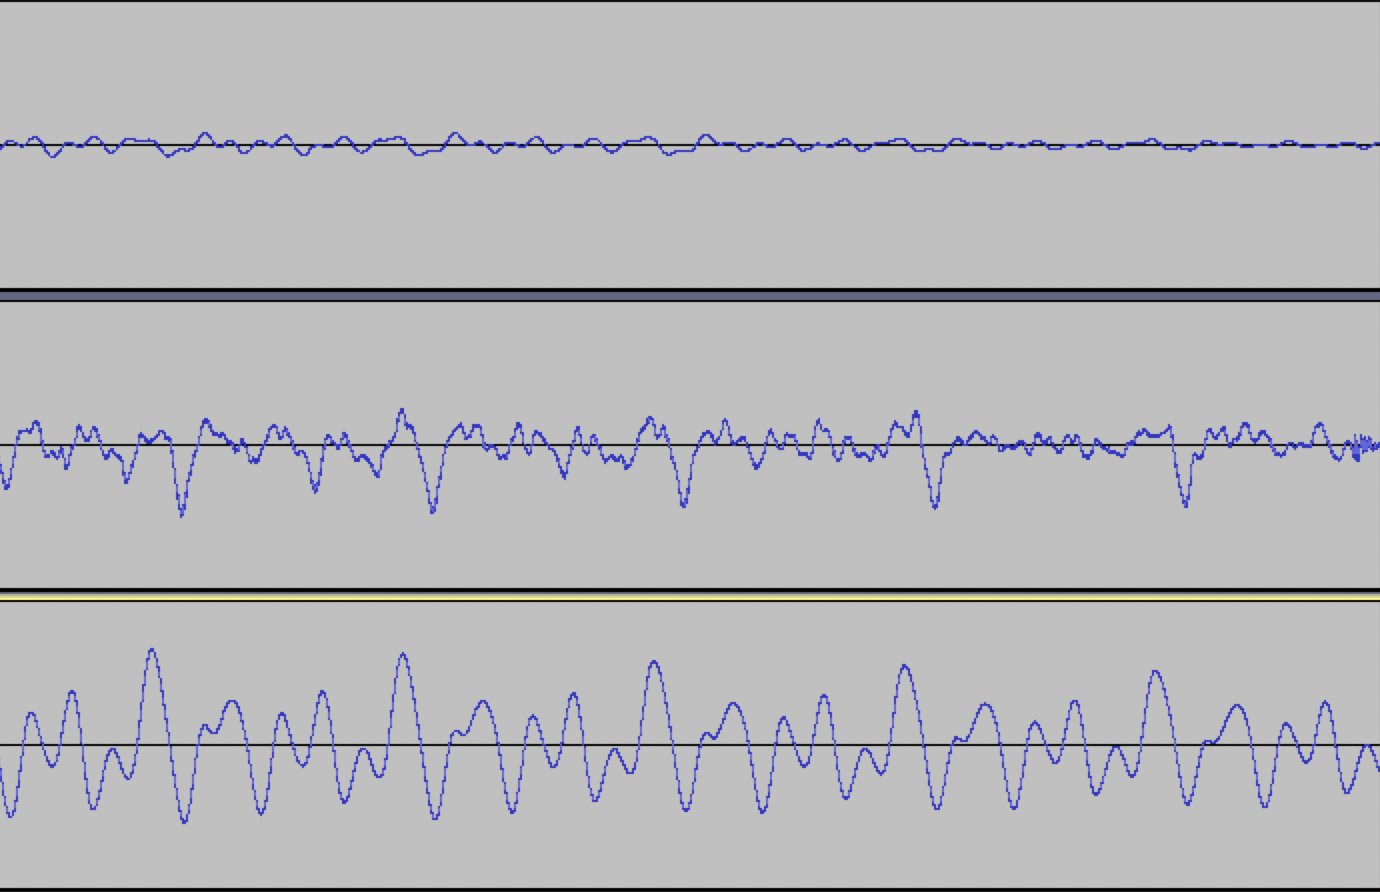
\includegraphics[width=0.85\columnwidth]{figure/88_88_det/a0_0800_1000.png}
\caption[A0の音波]{A0の0.800秒から1.000秒までの音波}
\label{fig:88_88_reduce1}
\end{minipage}
\begin{minipage}{0.48\columnwidth}
\centering
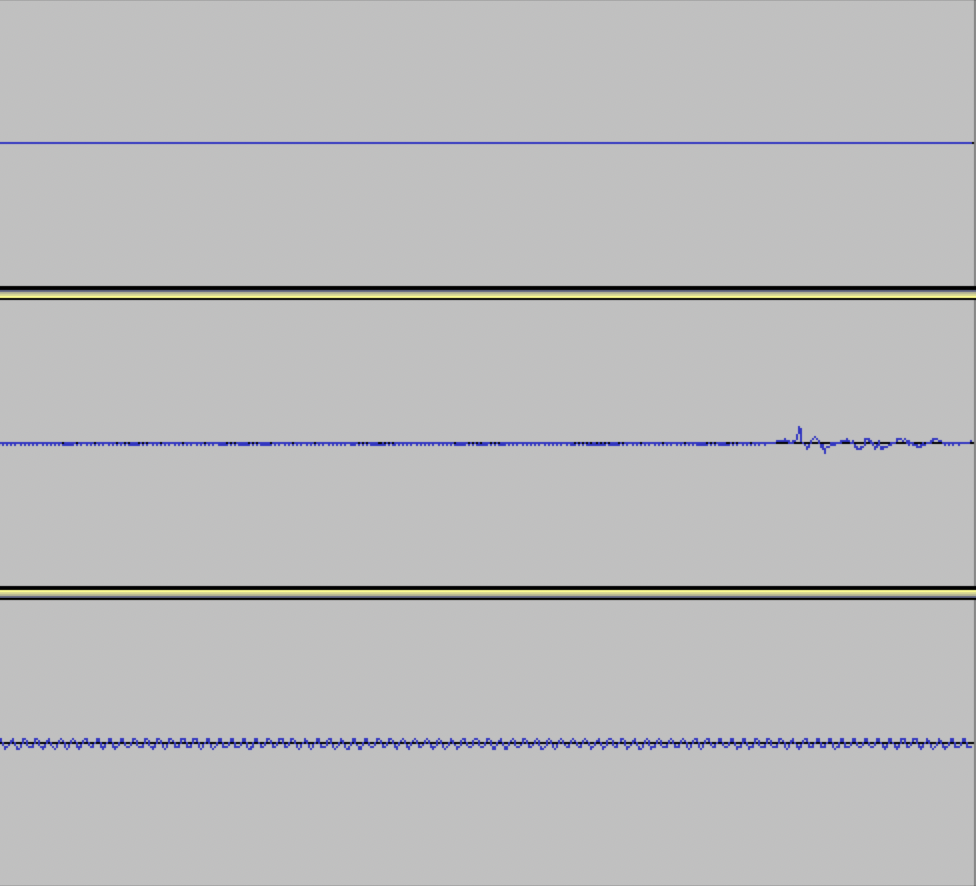
\includegraphics[width=0.75\columnwidth]{figure/88_88_det/b7_0980_1000.png}
\caption[B7の音波]{B7の0.980秒から1.000秒までの音波}
\label{fig:88_88_reduce2}
\end{minipage}
\end{figure}

%ここで改ページ
\clearpage

\subsubsection{音の大きさの維持}

部分的に大きさを維持できていない音がいくつかあった。\prettyref{fig:88_88_amp}では、波形の前半において生成波形の振幅が小さいことがわかる。原因は振幅をランダムに小さくしたことにあると考えられ、学習の初段階では振幅を固定しておくことや振幅の大きさを別で調整するなどの工夫が必要であると考えられる。
    
\subsubsection{音波の滑らかさの表現}

ノイズまじりの音がいくつかあった。これらの音を詳細に観察すると、生成された音波では滑らかさを表現できていないことがわかった~(\prettyref{fig:88_88_smooth})~。音波を滑らかにするような加工を生成後に加えるなどの工夫が必要であると考えられる。

\begin{figure}[b]
\centering
\begin{minipage}{0.48\columnwidth}
\centering
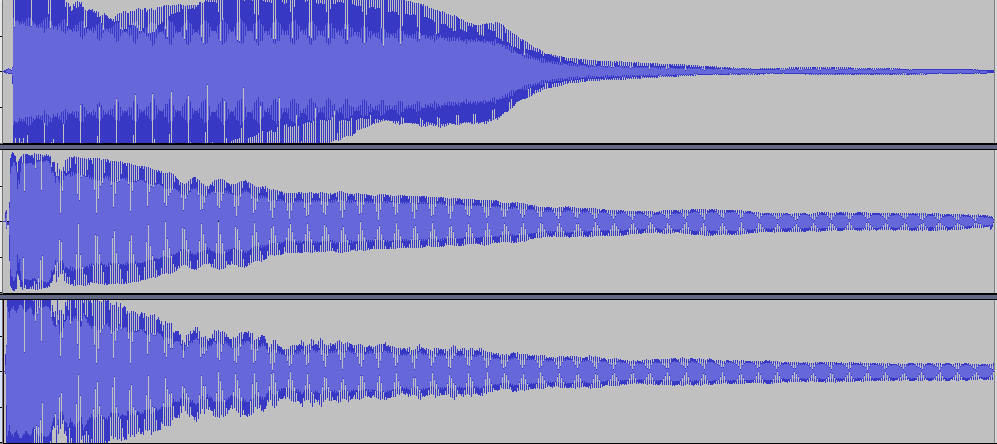
\includegraphics[width=0.85\columnwidth]{figure/88_88/c5.png}
\caption[C5の音波]{C5の0.000秒から1.000秒までの音波}
\label{fig:88_88_amp}
\end{minipage}
\begin{minipage}{0.48\columnwidth}
\centering
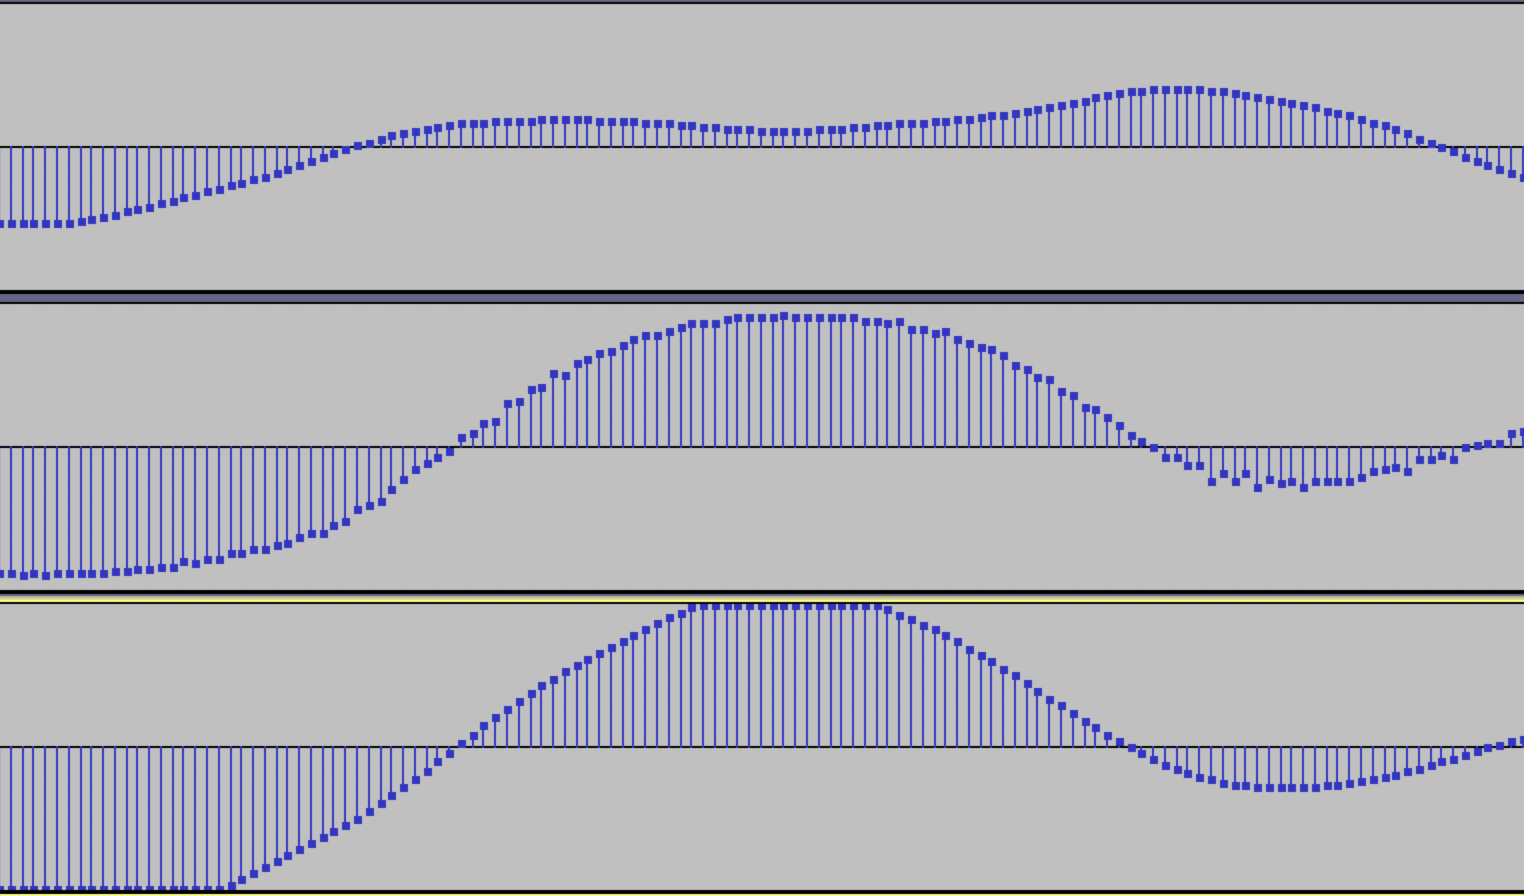
\includegraphics[width=0.75\columnwidth]{figure/88_88_det/d2s_0100_0103.png}
\caption[D2$\sharp$の音波]{D2$\sharp$の0.100秒から0.103秒までの音波}
\label{fig:88_88_smooth}
\end{minipage}
\end{figure}

\subsubsection{データセットの不安定さ}

ここまでの三つは提案モデルの改善により解消されると考えられるが、問題のあるデータセットも一部に存在した。一つの問題点は高音において振動が不安定になることであり、ここまでで述べた。もう一つの問題点は音の鳴り出しでの振動が不安定であるという点である。具体的には、\prettyref{fig:88_88_lag1}のようにギターの音の鳴り出しの遅延の方がハープより大きい場合や\prettyref{fig:88_88_lag2}のように周期的な音になるまでに遅延があるために不規則な振動となる場合などがあった。

\begin{figure}[b]
\centering
\begin{minipage}{0.48\columnwidth}
\centering
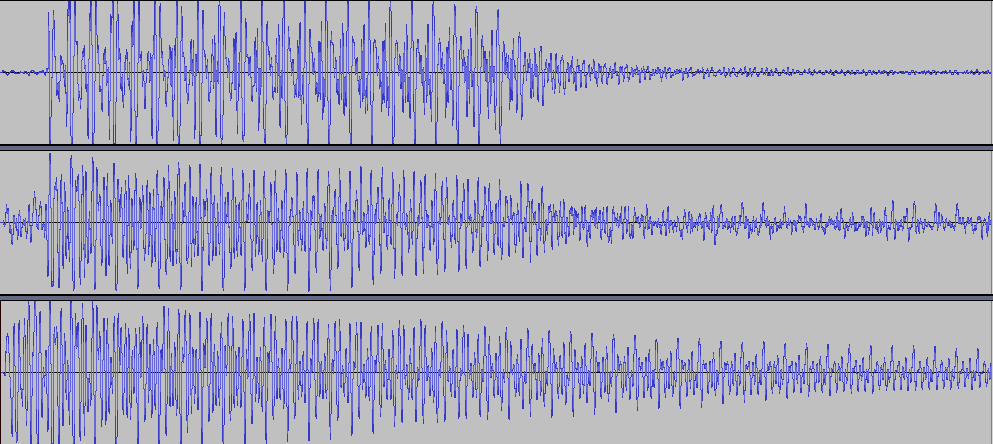
\includegraphics[width=0.9\columnwidth]{figure/88_88/f1s.png}
\caption[F1$\sharp$の音波]{F1$\sharp$の0.000秒から1.000秒までの音波}
\label{fig:88_88_lag1}
\end{minipage}
\begin{minipage}{0.48\columnwidth}
\centering
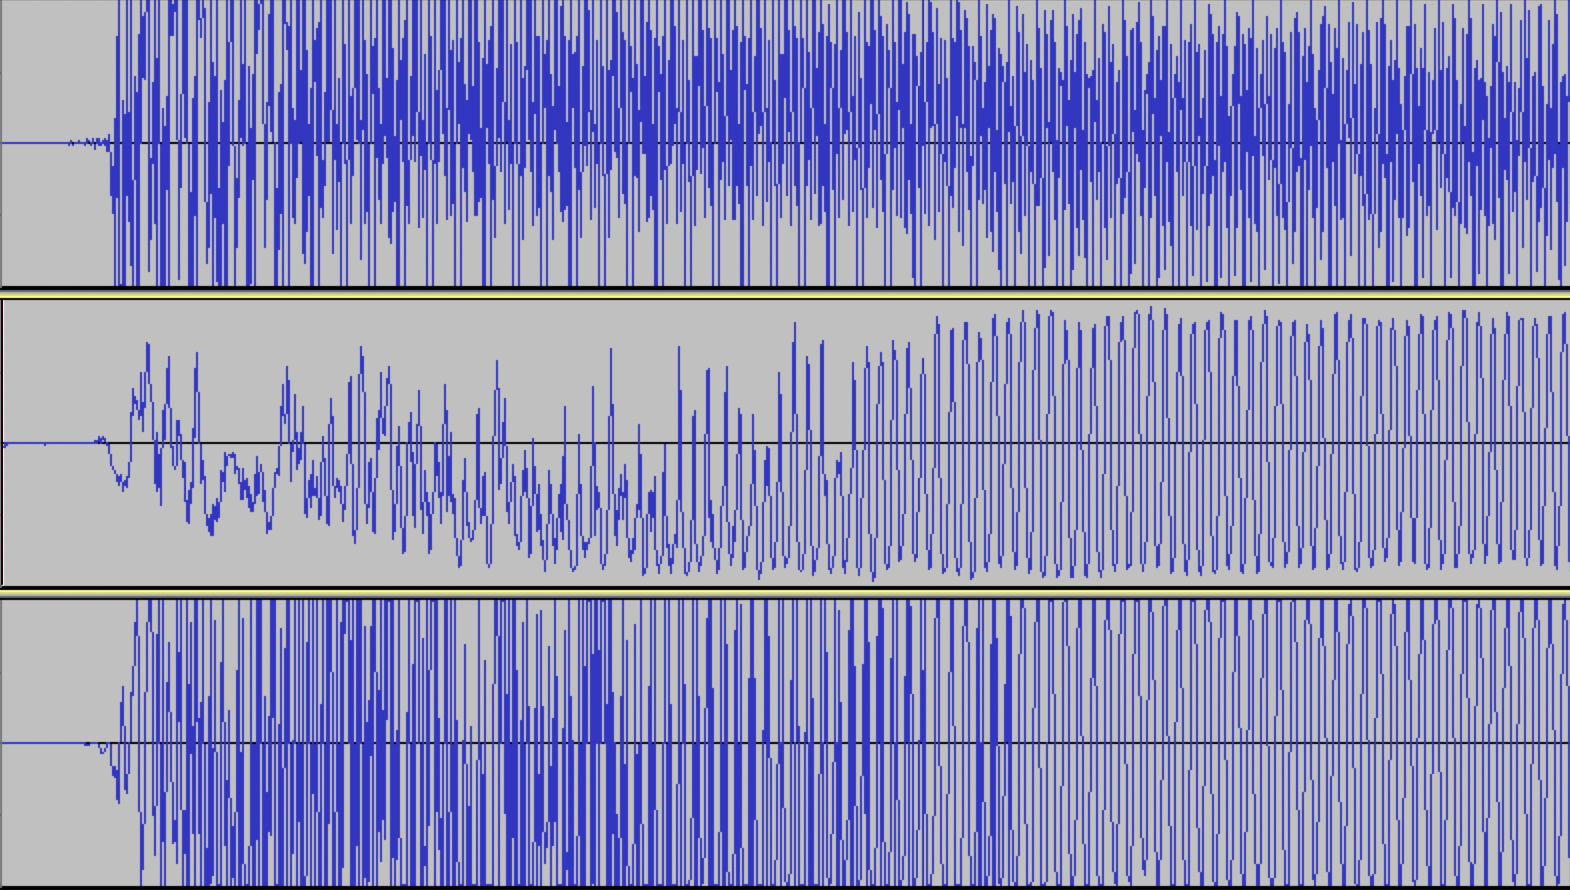
\includegraphics[width=0.75\columnwidth]{figure/88_88_det/a7_0_0030.png}
\caption[A7の音波]{A7の0.000秒から0.030秒までの音波}
\label{fig:88_88_lag2}
\end{minipage}
\end{figure}